% ---------------------------------------------------------------
% TO COMPILE USE: pdflatex -shell-escape -jobname report *.tex
% ---------------------------------------------------------------

\documentclass[12pt,a4paper]{article}

% ---------------------------------------------------------------
% ALL PACKAGES
% ---------------------------------------------------------------
\usepackage[left=3cm,right=2.5cm,top=3cm,bottom=2.5cm]{geometry}
\usepackage[utf8]{inputenc}
\usepackage[portuguese]{babel}
\usepackage{indentfirst}
\usepackage{graphicx}
\usepackage{hyperref}
\usepackage{caption}
\usepackage{subcaption}
\usepackage{listings}
\usepackage{enumitem}
\usepackage{float}
\usepackage{color}
\usepackage{booktabs}
\usepackage[dvipsnames,table,xcdraw]{xcolor}
\usepackage{url}
\usepackage{amsmath}
\usepackage{mathabx}
\usepackage{mathtools}
\usepackage{outlines}
\usepackage[normalem]{ulem}
\usepackage{adjustbox}

\usepackage{minted} %for code template
\usemintedstyle{friendly}
\definecolor{bg}{rgb}{0.96,0.96,0.96}





\begin{document}
% ---------------------------------------------------------------
% FIRST PAGE
% ---------------------------------------------------------------
\begin{titlepage}
    \centering
    \begin{figure}[H]
        \centering
        
\includegraphics[scale=2.2]{images/logo_um.jpg}
    \end{figure}
    {\huge\bfseries Universidade do Minho \par}
    \vspace{0.5cm}
    {\large Mestrado Integrado em Engenharia Informática \par}
    \vspace{2cm}
    {\Large \emph{System Deployment and Benchmarking} \par}
    \vspace{2cm}
    {\Large Fase 1 \par}
    \vspace{0.2cm}
    {\Large\bfseries \emph{Deployment} da aplicação \emph{GitLab} \par}
    \begin{figure}[H]
        \centering
        
\includegraphics[scale=0.5]{images/gitlab_logo.png}
    \end{figure}
    \vspace{2.5cm}
    {\Large Grupo 4 \par}
     \vspace{0.5cm}
    {\Large\itshape João Alves (A77070)\par}
    {\Large\itshape Gonçalo Raposo (A77211)\par}
    {\Large\itshape Alexandre Dias (A78425)\par}
    {\Large\itshape Hugo Oliveira (A78565)\par}
    \vfill
    {\large \today\par}
    \centering
\end{titlepage}




% ---------------------------------------------------------------
% ABSTRACT
% ---------------------------------------------------------------
\vspace*{\fill}
\begin{abstract}
No presente relatório vai ser feita uma análise do \textit{GitLab}. Será feita uma breve explicação sobre o que consiste a aplicação e qual a sua funcionalidade, posteriormente irá ser descrita a arquitetura do \textit{GitLab} e serão analisados os diferentes componentes da aplicação, assim como a sua função e importância.

Analisar-se-á ainda os ficheiros de configuração do \textit{GitLab} de forma a perceber as diferentes formas de implementação e integração de diferentes componentes da aplicação, como HAProxy e Unicorn. Serão ainda analisados os componentes críticos da aplicação e diferentes implementações de disponibilidade juntamente com as vantagens e desvantagens das mesmas.
\end{abstract}
\vspace*{\fill}
\thispagestyle{empty}




% ---------------------------------------------------------------
% TABLE OF CONTENTS
% ---------------------------------------------------------------
\clearpage
\tableofcontents
\listoffigures
\clearpage




% ---------------------------------------------------------------
% INTRODUCTION
% ---------------------------------------------------------------
\setcounter{page}{1}
\section{Introdução}
Hoje em dia, grande parte da população prescinde de algum do seu tempo em deslocações de e para os seus locais de trabalho, e espera-se que permaneçam no seu escritório, cumprindo assim os seus horários estabelecidos nos contratos. No entanto, apesar de já existirem várias empresas que são remote-friendly, o \emph{GitLab}, adotou uma ideia bastante diferente na sua organização, e abandonou o conceito de escritório físico permanentemente.
\newline
\par Numa primeira fase, iremos apresentar a plataforma \emph{GitLab} e por sua vez os serviços oferecidos por esta.Posteriormente iremos demonstrar toda a arquitetura do \emph{GitLab} primeiro fazendo uma comparação desta com um escritório físico e mais tarde descrevendo cada componente no que diz respeito às suas funcionalidades incluindo Base de Dados e Gestor de ficheiros.Seguidamente, será relatado sobre os ficheiros de configuração da plataforma assim como forma de editar estes e comandos associados.No quinto capítulo, serão expostos os componentes críticos do \emph{GitLab}. Finalmente, no ultimo capítulo, serão apresentados várias implementações do sistema consoante a Disponibilidade necessária para satisfazer os serviços de diferentes números de utilizadores, variando das dezenas até às centenas de milhares. 






% ---------------------------------------------------------------
% CONTENT
% ---------------------------------------------------------------
\newpage
\section{\emph{GitLab}}
Antes de podermos descrever toda a arquitetura e funcionamento do \emph{GitLab}, é necessário perceber o que é o \emph{\textbf{git}}.

\subsection{O que é o \emph{git}?}
O \emph{git} é um sistema \emph{open source} que permite controlar versões de ficheiros de um projecto de uma forma rápida e eficaz.

O uso de um sistema como este, permite, em projetos que possam envolver vários contribuidores, criar e editar ficheiros em simultâneo, bem como retroceder a versões mais antigas destes. Assim, existe a possibilidade de analisarmos toda a evolução de um projecto.

\subsection{O que é o \emph{GitLab}?}
O \textbf{\emph{GitLab}} é uma plataforma grátis que permite hospedar projectos em servidores locais ou remotos, utilizando o \textbf{\emph{git}} para fazer o controlo de versões. O \emph{GitLab} é um concorrente \emph{open source} direto aos serviços \emph{GitHub} e \emph{Bitbucket}.

Para além desta sua principal funcionalidade, a empresa \emph{GitLab} disponibiliza o código da sua aplicação para que qualquer utilizador possa a usar livremente num outro ambiente. Recentemente, foi disponibilizado uma imagem \emph{Docker} que permite instalar e correr o \emph{GitLab} facilmente. Para uma utilização que permita uma alta disponibilidade da aplicação, é necessário alterar e configurar os diferentes componentes da \emph{stack} aplicacional do \emph{GitLab}.

\subsection{\emph{GitLab Software Delivery}}
Existem atualmente dois tipos de distribuição do \emph{GitLab}, a versão CE (\emph{Community Edition}) e a versão EE (\emph{Enterprise Edition}).

\begin{itemize}
    \item \textbf{\emph{Community Edition}}: é uma versão \emph{open source} onde não apoio de uma qualquer empresa no processo de \emph{delivery} ou \emph{deployment}. Apresenta funcionalidades reduzidas.
    \item \textbf{\emph{Enterprise Edition}}: ao contrários da versão anterior, esta inclui vários serviços para além dos incluidos na versão CE, entre estes, destacamos o suporte técnico especializado 24/7, a gestão adicional de servidores, \emph{performance} e segurança, ferramentas de estatística. Esta versão apresenta diferentes preçários mensais.
\end{itemize}












% ---------------------------------------------------------------
\newpage
\section{Arquitetura do \emph{GitLab}}\label{arq}

A alta \textbf{disponibilidade} e \textbf{escabilidade} são, hoje em dia, condições importantes e obrigatórias em qualquer aplicação. Se estes requisitos não são cumpridos, os utilizadores podem querer migrar para outra aplicação idêntica.

Um dos principais aspetos para a alta disponibilidade, consiste no \emph{clustering} da aplicação. Isto é, para prevenirmos que uma aplicação se torne indisponível, são criadas várias réplicas da mesma. Estas réplicas são, no entanto, invisiveis ao utilizador, dado que este apenas vê a aplicação como uma única instância.

Seguindo este raciocinio, o \emph{GitLab} foi desenhado sobre um padrão de várias camadas a trabalhar entre si. Como hoje em dia é impossível tornar uma aplicação \emph{stateless}, devido à necessidade de armazenamento de informações, é importante separarmos os componentes com estado (como uma base de dados ou sistema de ficheiros) dos componentes sem estado, meramente aplicacionais. Como seria de esperar, isto gera complexidade no desenho e configuração da aplicação.

O \emph{GitLab} possui cerca de 7 camadas aplicacionais distintas, projetadas e configuradas para assegurarem a alta disponibilidade. A imagem em baixo, demonstra a arquitetura do \emph{GitLab}.

\begin{figure}[H]
  \centering
  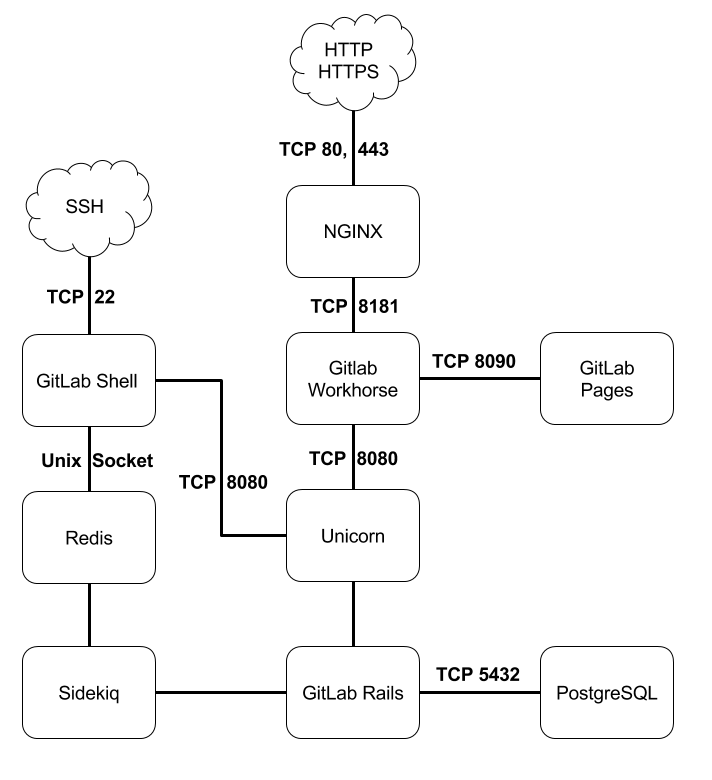
\includegraphics[scale=0.47]{images/gitlab_architecture_diagram.png}
  \caption{Arquitetura do \emph{GitLab}.}
\end{figure}

% ---------------------------------------------------------------
\newpage
\subsection{A arquitetura vista como um escritório físico}

Toda a estrutura do \emph{GitLab} pode ser comparada como um escritório físico. Vejamos alguns componentes na seguinte lista.

\begin{itemize}
    \item \textbf{Os repositórios} serão os bens que o \emph{GitLab} gere. Estes armazenam as chamadas \textit{codebases}, que são constituídas por todo o código fonte que é usado para construir uma aplicação;
    \item \textbf{\emph{Nginx}} pode ser visto como uma secretaria, onde os utilizadores se dirigem para requisitar certas operações, que serão realizadas pelos funcionários que lá trabalham;
    \item \textbf{Armazenamento de dados} consiste numa série de armários que contêm ficheiros com informações sobre:
    \begin{itemize}
        \item os bens que são armazenados;
        \item os utilizadores que se dirigem à secretaria.
    \end{itemize}
    \item \textbf{\emph{Redis}} é visto como uma espécie de quadro, que contém uma série de tarefas, para serem executadas pelos funcionários;
    \item \textbf{\emph{Sidekiq}} pode ser comparado como um trabalhador, que recolhe as suas tarefas do quadro (\emph{Redis}), tratando principalmente do envio de emails;
    \item \textbf{\emph{Unicorn worker}} é um operário que trata de tarefas rápidas/gerais, coletadas pelo quadro (Redis). Estas consistem principalmente em:
    \begin{itemize}
        \item verificar as permissões dos utilizadores , confirmando a sessão de cada um no \emph{Redis};
        \item criar tarefas para o \emph{Sidekiq};
        \item recolher dados presentes no armazenamento de dados.
    \end{itemize}
    \item \textbf{\emph{GitLab-shell}} pode ser visto também como um funcionário que recebe ordens (por \emph{SSH}), comunica com o \emph{Sidekiq} por via do \emph{Redis} e faz alguns pedidos rápidos aos \emph{Unicorn Workers} ou diretamente, ou por via do \emph{Nginx};
    \item \textbf{\emph{Gitaly}} corresponde a uma espécie de escritório secundário que gere todas as operações feitas através do \emph{git}, desde monitorizar a sua eficiência, até manter cópias dos resultados de operações mais custosas.
\end{itemize}

Com esta simples introdução aos componentes da arquitetura do \emph{GitLab}, conseguimos visualizar o seu funcionamento.

Nas secções a seguir, serão descritos todos os componentes presentes na arquitetura do \emph{GitLab}.


% ---------------------------------------------------------------
\subsection{\emph{GitLab frontend}}

A aplicação \emph{GitLab} apresenta uma interface \emph{web} que utiliza várias tecnologias \emph{open source}. A sua aplicação \emph{web} foi desenvolvida utilizando a \emph{framework} \emph{Ruby on Rails}, baseada num padrão \emph{MVC}. Esta aplicação permite não só, a gestão de repositórios \emph{git}, como também a gestão de comentários, que complementam os diferentes projetos.

Relativamente à estruturação da aplicação \emph{web}, é importante destacarmos os seguintes componentes da camada aplicacional:

\begin{itemize}
    \item \emph{\textbf{NGINX}}: é um servidor \emph{web} utilizado para servir conteúdo \emph{web} aos clientes;
    \item \emph{\textbf{GitLab Shell}} e \emph{\textbf{GitLab Workhorse}}: lidam com os comandos \emph{git} enviados pela a aplicação \emph{web} ou por conexões via \emph{ssh}. Ou seja, comandos como \emph{clone, fork, push} ou \emph{pull}, são redirecionados para um destes componentes, onde serão executados;
    \begin{itemize}
        \item o \emph{GitLab Shell} permite ainda modificar a lista as chaves autoritativas \emph{ssh} dos utilizadores, verificar um determinada chave pública, limitar comandos \emph{git} aos utilizadores e, por fim, copiar entre o cliente e servidores \emph{Gitaly};
        \item o \emph{GitLab Workhorse} funciona como um \emph{reverse proxy} que trata de pedidos \emph{http} (p.e transferências de arquivos, \emph{git pull/push}, etc). É responsável por assumir uma ligação direta com a aplicação \emph{GitLab}, tentando sempre que possível, diminuir as comunicações entre estes dois (por exemplo ficheiros \emph{Javascript} e \emph{CSS} são diretamente passados ao cliente); assume-se então que os servidores \emph{Nginx} ou \emph{Apache} enviam os pedidos ao \emph{Workhorse} e este ao \emph{backend} do \emph{GitLab}.
    \end{itemize}
    \item \emph{\textbf{Sidekiq}}: ferramenta responsável pela gestão e execução de processos \emph{Ruby} da aplicação \emph{GitLab} em \emph{background}. O \emph{Sideiq} foi introduzido devido a \emph{memory leaks} da aplicação \emph{GitLab}. Ou seja, por forma a evitar as fugas de memória, o \emph{Sideiq} é reiniciado a cada intervalo de tempo previamente definido, permitindo que a aplicação esteja disponível;
    \item \emph{\textbf{Unicorn}}: tal como o \emph{Sideiq}, o \emph{Unicorn} foi introduzido para gerir e uso de memória entre pedidos \emph{web http} e pedidos \emph{git} via \emph{http}. É um \emph{deamon} que corre a aplicação \emph{GitLab} (\emph{master}) e contém um conjuntos de \emph{workers}. Cada um é responsável por executar uma tarefa durante um determinado período (\emph{timeout}, caso contrário, a tarefa é atribuída a outro \emph{worker}. O \emph{master} nunca lida com os pedidos recebidos. Tal como referido anteriormente, o \emph{GitLab} apresenta \emph{memory leaks}. Ao fim de algum tempo, os processos começam a apresentar falhas, que podem ser controladas com a interropção do processo (\emph{kill}).
\end{itemize}

Os componentes descritos em cima fazem parte da camada aplicacional \emph{GitLab}, no entanto, não traduzem a verdadeira essência da aplicação \emph{GitLab}. Isto é, a aplicação ou várias instâncias desta não guardam qualquer tipo de informação a longo prazo. O \emph{frontend} do \emph{GitLab} faz pedidos à camada lógica da aplicação para que possa ser guardado um dado estado ou informação num dos outros componentes da \emph{stack}. O único estado que é guardado na aplicação, é o ficheiro de configuração que abordaremos mais à frente.

\subsubsection{\emph{HAProxy}}

% Tal como foi referido no início da secção \pageref{arq}, o \emph{GitLab} foi desenhado com o intuito de tornar a sua aplicação e os seus serviços altamente disponíveis ao público alvo.

O \emph{HAProxy} (\emph{High Performance TCP/HTTP Load Balancer}) é um servidor \emph{proxy} para \emph{web} que oferece soluções fiáveis como: alta escalabilidade, balanceamento de carga e \emph{proxying} para aplicações que usam \emph{TCP} e \emph{HTTP}.

No contexto da aplicação \emph{GitLab}, o \emph{HAProxy} tem várias funcionalidades e funciona como um \emph{gateway} que distribui tráfego e pedidos pelos vários servidores que correm a aplicação \emph{GitLab}. Em baixo, encontra-se uma imagem que pretende demonstrar o funcionamento do \emph{HAProxy}, destacado como \emph{load balancer} que recebe vários pedidos \emph{SSH} e \emph{HTTP} e encaminha-os para os servidores que correm o \emph{GitLab}.

\begin{figure}[H]
  \centering
  \includegraphics[scale=0.25]{images/haproxy.png}
  \caption{Exemplo de funcionamento do \emph{HAProxy}.}
\end{figure}

Para além das funcionalidades descritas em cima, o \emph{HAProxy} funciona como um \emph{edge-node} entre a rede externa (\emph{internet}) e a rede interna do \emph{GitLab}. Isto é, o \emph{HAProxy} irá negar qualquer tentativa de acesso (através de \emph{sockets unix}) aos servidores \emph{frontend} do \emph{GitLab}.

% Relativamente à comunicação entre os vários servidores \emph{proxy} e os servidores aplicacionais, existem três formas distintas: os servidores aplicacionais detêm o seu próprio \emph{SSL} (um distinto para cada servidor);
% https://docs.gitlab.com/ee/administration/high_availability/load_balancer.html

\subsubsection{\emph{Keepalived}}

Juntamente com o \emph{HAProxy}, existe a aplicação \emph{Keepalived} que garante que o serviço \emph{GitLab} está sempre disponivel. Isto é, permanece ativas duas instâncias idênticas do \emph{HAProxy}, garantido assim, que pelo menos uma delas se encontra configurada para um determinado IP, tornando o \emph{HAProxy} eficiente. Se uma instância falhar, outra é automaticamente configurada para o IP anterior (único).



\subsection{\emph{Redis}}

O \emph{Redis} funciona como uma estrutura de armazenamento de dados guardada em memória. É geralmente utilizado para fazer \emph{caching} de dados que, na maioria das vezes, permanecem em memória num curto período de tempo.

Dentro da camada aplicacional do \emph{GitLab}, o \emph{Redis} funciona como um serviço que guarda as sessões ativas de utilizadores e uma lista de tarefas a serem realizadas pelo \emph{Sidekiq}. Isto é, a informação da sessão de um utilizador e as tarefas que estão a ser executadas são guardadas numa ou várias instâncias \emph{Redis}.

Para além destas funcionalidades, o \emph{Redis} permite que os restantes componentes da camada aplicacional guardem o seu estado e o partilhem com o resto dos componentes, por exemplo, através de trocas de messagens. Tal como alguns dos componentes anteriores, é também importante que toda a informação seja consistente e facilmente partilhada com as várias instâncias do \emph{GitLab}.

\subsubsection{\emph{Redis Sentinel}}

O \emph{Redis Sentinel} tem uma funcionalidade muito semelhante ao \emph{Keepalived}. Para garantirmos uma alta disponibilidade, é necessário que para além de existir um \emph{Master} e um \emph{Slave} do \emph{Redis}, exista algo à escuta de falhas de instâncias \emph{Redis}, começando automaticamente o processo de \emph{failover}, que consiste em atribuir uma nova instância aquando uma falha.

Com o \emph{Redis Sentinel}, consegue-se garantir a existência e disponibilidade de uma instância \emph{Redis} para um cliente, tornando abstratas todas as falhas.




\subsection{Base de dados - \emph{PostgreSQL}}
O \emph{Postegres} é um sistema de base de dados relacional \emph{open source} que permite o controlo e  persistência de dados.

Os dados que são armazenados incluem dados do utilizador (como \emph{username}, \emph{email}, \emph{password}, definições de conta, etc), permissões dos repositórios, comentários, problemas encontrados e todos os outros dados que não são diretamente controlados pelo \emph{git}. Todos os dados devem, uma vez mais, estar disponíveis e consistentes para poderem ser exibidos e validados corretamente para a aplicação \emph{web} do \emph{GitLab}.

Num cluster onde possam existir várias instâncias do \emph{Postgres} (como o \emph{master} ou \emph{slaves}/réplicas), existe também uma instância do \emph{HAProxy}. Tal como vimos anteriormente, o \emph{HAProxy} permite o balanceamento de carga e permite transmitir os pedidos a um grupo de nós previamente conhecidos. Ou seja, qualquer instância da aplicação \emph{GitLab} irá comunicar com este \emph{HAProxy} acreditando que este é a base de dados. 

Os diferentes \emph{slaves} são configurados para se manterem \emph{up to date} e prontos a atuarem como \emph{master} no caso de uma falha do servidor principal. A alta escalabilidade e disponibilidade do \emph{Postgres} é mantida através da utilização de instâncias \emph{HAProxy} e \emph{Patroni}.


\subsubsection{\emph{Patroni}}

O \emph{Patroni} é uma \emph{framework} escrita em \emph{python} usada para facilitar e automatizar processos como replicação e falhas de instâncias do  \emph{PostgreSQL}.

Ainda que o \emph{Postreges} suporte mecanismos de \emph{master/slave}, a adição ou remoção de novos nós que contêm réplicas dos dados é uma tarefa dificil e que requer configurações que podem induzir a erros. Com a integração do \emph{Patroni}, é possivel utilizar aplicar estes mecanismos de replicação automaticamente sem necessidade dos habituais processos manuais de configuração. Além disso, após uma falha, o \emph{Patroni} é capaz de resolver o processo de recuperação, selecionando um novo \emph{master}.

Esta \emph{framework} corre em conjunto com as instâncias do \emph{Postgres}. Para que seja possível reconhecer e atualizar o estado de cada uma destas instâncias, o \emph{Patroni} recorre ao \emph{ETCD}, no entanto este suporta outras alternativas, como \textbf{\emph{Consul}} ou \textbf{\emph{Zookeeper}}.

\begin{figure}[H]
\begin{minted}[bgcolor=bg, 
               fontsize=\footnotesize, 
               framesep=2mm,
               % linenos,
               breaklines,
               breakautoindent=true,
               breaksymbolleft=\raisebox{0.8ex}{\tiny\hookrightarrow},
               breaksymbolindentleft=0pt,
               breaksymbolsepleft=1pt,
               breaksymbolright=\raisebox{0.8ex}{\tiny\hookleftarrow},
               breaksymbolindentright=0pt,
               breaksymbolsepright=1pt
]{text}
+---------------+--------+-------------+--------+----------+-----------+
|    Cluster    | Member |     Host    |  Role  |  State   | Lag in MB |
+---------------+--------+-------------+--------+----------+-----------+
| pg-ha-cluster |  pg-1  | 10.142.0.11 |        | running  |       0.0 |
| pg-ha-cluster |  pg-2  | 10.142.0.10 | Leader | running  |       0.0 |
| pg-ha-cluster |  pg-3  | 10.142.0.09 |        | running  |       0.0 |
+---------------+--------+-------------+--------+----------+-----------+
\end{minted}
\caption{Exemplo de uma tabela com o estado do \emph{Patroni}.}
\label{fig:c}
\end{figure}


\subsection{\textcolor{red}{Gestores de ficheiros} - reformular}

Todas as instâncias do \emph{GitLab} que necessitam de acesso ao mesmo sistema de ficheiros, utilizam o \emph{git}. O \emph{git} é um software de gestão e controlo de versões, direcionado principalmente para código fonte, cujo protocolo funciona guardando ficheiros num sistema de ficheiros partilhado. No entanto, existem também algumas outras pastas que são partilhadas fora do \emph{git}. Incluem-se: a pasta que armazena as chaves \emph{SSH}, recursos estáticos que são carregados (como é o de imagens) e outros ficheiros que necessitam de estar presentes em todas as instâncias do \emph{GitLab}.

\bigbreak
% ver https://gist.github.com/yurishkuro/10cb2dc42f42a007a8ce0e055ed0d171
Ferramentas como \textbf{\emph{ETCD}}, \textbf{\emph{Consul}} e \textbf{\emph{Zookeeper}} permitem guardar informações num estilo \emph{key-value} dentro de um \emph{cluster}. Ou seja, podemos guardar o estado de cada uma das instâncias do \emph{Postegres} nestas ferramentas. 

Consideremos o \emph{ETCD}. Este aprensenta um \emph{time to live} (configurável) para o armazenamento dos dados. Isto é, ao fim deste tempo, todos os dados sobre os estados das máquinas, é removido. Isto garante que as instâncias \emph{Patroni} verificam continuamente o estado e o atualizam. Com a utilização deste recurso, o \emph{Patroni} consegue reconhecer facilmente quem são as máquinas disponíveis bem como o líder atual. Como podemos verificar, este é um componente crítico na estrutura do \emph{GitLab}, pelo que devem existir várias instâncias de \emph{ETCD}.



\subsection{\emph{Gitaly}}

O \emph{Gitaly} é um serviço RPC (\emph{Remote Procedure Call}) que trata todas as chamadas ao \emph{git}, feitas pelo \emph{GitLab}.

O diagrama seguinte mostra como um servidor \emph{git} teria um número de clientes distintos.

\begin{figure}[H]
  \centering
  \includegraphics[scale=0.4]{images/gitlab-gitaly.png}
  \caption{Exemplo de }
\end{figure}

Mas eu não acho que seja aquilo que se tem que falar



% ---------------------------------------------------------------
\newpage
\section{Ficheiros de configuração}

Para uma melhor interpretação do ficheiro de configuração, utilizamos o \emph{Omnibus}, um \emph{package} de instalação do \emph{GitLab} para podermos configurar os parâmetros da aplicação \emph{GitLab} diretamente.

O ficheiro principal de configuração é o \texttt{gitlab.rb}. Cada instância do \emph{GitLab} irá possuir o seu ficheiro de configuração. Este ficheiro encontra-se na seguinte diretoria:

\begin{minted}[bgcolor=bg, 
               fontsize=\footnotesize, 
               framesep=2mm,
               breaklines,
               breakautoindent=true,
               breaksymbolleft=\raisebox{0.8ex}{\tiny\hookrightarrow},
               breaksymbolindentleft=0pt,
               breaksymbolsepleft=1pt,
               breaksymbolright=\raisebox{0.8ex}{\tiny\hookleftarrow},
               breaksymbolindentright=0pt,
               breaksymbolsepright=1pt
]{text}
/etc/gitlab/
\end{minted}

Sempre que for efetuada qualquer alteração neste ficheiro, devemos executar o seguinte comando:
\begin{minted}[bgcolor=bg, 
               fontsize=\footnotesize, 
               framesep=2mm,
               breaklines,
               breakautoindent=true,
               breaksymbolleft=\raisebox{0.8ex}{\tiny\hookrightarrow},
               breaksymbolindentleft=0pt,
               breaksymbolsepleft=1pt,
               breaksymbolright=\raisebox{0.8ex}{\tiny\hookleftarrow},
               breaksymbolindentright=0pt,
               breaksymbolsepright=1pt
]{bash}
$ gitlab-ctl reconfigure
\end{minted}

De seguida, iremos abordar algumas das possíveis configurações que são permitidas no \emph{GitLab}.


% ---------------------------------------------------------------
\subsection{Endereço \emph{url} para acesso ao \emph{GitLab}}

Para que os utilizadores consigam aceder remotamente à aplicação \emph{web} do \emph{GitLab}, é necessário definir o \emph{url}. De notar que, caso pretendam um acesso externo, é necessário registar este endereço \emph{url} para que seja possível a resolução de nomes (DNS), ou seja, associar este \emph{ip} ao nome. 

Para isto, basta adicionar a seguinte linha ao ficheiro de configuração:

\begin{minted}[bgcolor=bg, 
               fontsize=\footnotesize, 
               framesep=2mm,
               breaklines,
               breakautoindent=true,
               breaksymbolleft=\raisebox{0.8ex}{\tiny\hookrightarrow},
               breaksymbolindentleft=0pt,
               breaksymbolsepleft=1pt,
               breaksymbolright=\raisebox{0.8ex}{\tiny\hookleftarrow},
               breaksymbolindentright=0pt,
               breaksymbolsepright=1pt
]{ruby}
external_url "http://gitlab.example.com"
\end{minted}

É ainda possível definir um \emph{url} relativo: 

\begin{minted}[bgcolor=bg, 
               fontsize=\footnotesize, 
               framesep=2mm,
               breaklines,
               breakautoindent=true,
               breaksymbolleft=\raisebox{0.8ex}{\tiny\hookrightarrow},
               breaksymbolindentleft=0pt,
               breaksymbolsepleft=1pt,
               breaksymbolright=\raisebox{0.8ex}{\tiny\hookleftarrow},
               breaksymbolindentright=0pt,
               breaksymbolsepright=1pt
]{ruby}
external_url "http://example.com/gitlab"
\end{minted}


% ---------------------------------------------------------------
\subsection{Integração com a base de dados}

Como foi abordado anteriormente, o sistema de base de dados recomendado é o \emph{PostgreSQL}. 

Caso se pretenda utilizar uma máquina diferente para correr um sistema de base de dados, é necessário efetuar os seguintes passos:

\begin{itemize}
    \item \texttt{db\_host}: representa o \emph{ip} ou nome do nó/máquina;
    \item \texttt{db\_port}: representa a porta por onde está a ser fornecido o serviço \emph{postgres};
    \item \texttt{db\_database}: representa o nome do nome dado à base de dados;
    \item \texttt{db\_username} e \texttt{db\_password}: representa os dados de acesso à base de dados;
    \item \texttt{postgresql['enable']}: opção que permite desativar o \emph{postgres} nativo da aplicação, permitindo que seja outra instância a servi-la.
\end{itemize}

% gitlab_rails['db_encoding'] = "unicode"
% gitlab_rails['db_pool'] = 10

\begin{figure}[H]
\centering
\begin{minted}[bgcolor=bg, 
               fontsize=\footnotesize, 
               framesep=2mm,
               %linenos,
               breaklines,
               breakautoindent=true,
               breaksymbolleft=\raisebox{0.8ex}{\tiny\hookrightarrow},
               breaksymbolindentleft=0pt,
               breaksymbolsepleft=1pt,
               breaksymbolright=\raisebox{0.8ex}{\tiny\hookleftarrow},
               breaksymbolindentright=0pt,
               breaksymbolsepright=1pt
]{ruby}
gitlab_rails['db_adapter'] = "postgresql"
gitlab_rails['db_host'] = "10.0.0.101"  
gitlab_rails['db_port'] = 5432
gitlab_rails['db_database'] = "gitlab-prod"  
gitlab_rails['db_username'] = "gitlab-user"  
gitlab_rails['db_password'] = "gitlab-password"  

postgresql['enable'] = false
\end{minted}
\caption{Exemplo de configuração para o \emph{postgreSQL}.}
\label{fig:c}
\end{figure}

O \emph{package omnibus}, por \emph{default}, não irá importar o \emph{schema} da base de dados do \emph{GitLab} nem irá criar um administrador, necessário para a aplicação.

Como tal, é necessário proceder à criação da base de dados. É importante referir que este processo deverá ser apenas efetuado uma única vez, pelo que, os seguintes excertos de código apenas deverão ser adicionados num único ficheiro de configuração de um instância \emph{GitLab}.

\begin{minted}[bgcolor=bg, 
               fontsize=\footnotesize, 
               framesep=2mm,
               %linenos,
               breaklines,
               breakautoindent=true,
               breaksymbolleft=\raisebox{0.8ex}{\tiny\hookrightarrow},
               breaksymbolindentleft=0pt,
               breaksymbolsepleft=1pt,
               breaksymbolright=\raisebox{0.8ex}{\tiny\hookleftarrow},
               breaksymbolindentright=0pt,
               breaksymbolsepright=1pt
]{ruby}
# especificar uma password de utilizador root
gitlab_rails['initial_root_password'] = 'nonstandardpassword'
\end{minted}

Por fim, executar o comando \texttt{\$ gitlab-rake gitlab:setup}.

No caso de existirem vários servidores \emph{GitLab} a partilharem a mesma base de dados e for necessário efetuar a migração de dados de uma base de dados, é importante limitar o número de máquinas que irão efetuar este processo. Para isso devemos, para cada máquina que corre o \emph{GitLab}, adicionar o seguinte:

\begin{minted}[bgcolor=bg, 
               fontsize=\footnotesize, 
               framesep=2mm,
               %linenos,
               breaklines,
               breakautoindent=true,
               breaksymbolleft=\raisebox{0.8ex}{\tiny\hookrightarrow},
               breaksymbolindentleft=0pt,
               breaksymbolsepleft=1pt,
               breaksymbolright=\raisebox{0.8ex}{\tiny\hookleftarrow},
               breaksymbolindentright=0pt,
               breaksymbolsepright=1pt
]{ruby}
# ativar ou desativar a migração automática
gitlab_rails['auto_migrate'] = false
\end{minted}





% ---------------------------------------------------------------
\subsection{Integração com um servidor SMTP}

O \emph{GitLab} permite que seja utilizado um servidor de \emph{emails} externo, que esteja a correr noutro nó computacional.

Os parâmetros necessário à configuração são muito semelhantes aos da configuração de um servidor \emph{SMTP} ou \emph{IMAP}:

\begin{minted}[bgcolor=bg, 
               fontsize=\footnotesize, 
               framesep=2mm,
               %linenos,
               breaklines,
               breakautoindent=true,
               breaksymbolleft=\raisebox{0.8ex}{\tiny\hookrightarrow},
               breaksymbolindentleft=0pt,
               breaksymbolsepleft=1pt,
               breaksymbolright=\raisebox{0.8ex}{\tiny\hookleftarrow},
               breaksymbolindentright=0pt,
               breaksymbolsepright=1pt
]{ruby}
gitlab_rails['smtp_enable'] = true
gitlab_rails['smtp_address'] = "smtp.mailtrap.io"
gitlab_rails['smtp_port'] = 2525
gitlab_rails['smtp_user_name'] = "username"
gitlab_rails['smtp_password'] = "password"
gitlab_rails['smtp_domain'] = "smtp.mailtrap.io"
gitlab_rails['smtp_tls'] = true

gitlab_rails['smtp_openssl_verify_mode'] = 'none'
gitlab_rails['smtp_enable_starttls_auto'] = false
gitlab_rails['smtp_ssl'] = false
gitlab_rails['smtp_force_ssl'] = false
\end{minted}

O exemplo em cima está apenas a utilizar o protocolo de segurança \emph{TLS}, no entanto é possível utilizarmos também o protocolo \emph{SSL}.

O \emph{GitLab} disponibiliza \href{https://docs.gitlab.com/omnibus/settings/smtp.html#smtp-settings}{\emph{online}} vários exemplos de configuração de servidores \emph{SMTP} de vários \emph{providers}.


% ---------------------------------------------------------------
\subsection{Integração com o \emph{Nginx}}

Por \emph{default}, o \emph{package} de instalação \emph{omnibus} instala um \emph{bundle Nginx}. Para ser possível utilizar um conjunto de servidores externos \emph{Nginx} ou \emph{Apache}, é necessário os adicionar ao grupo de servidores \emph{web} \texttt{gitlab-www}.

Para se juntar novos servidores ao grupo descrito em cima, é necessário os adicionar ao grupo principal e, se necessário, desativar o \emph{bundle Nginx}. De notar que, para servidores que corram \emph{Debian/Ubuntu} o grupo será \texttt{www-data}. Para servidores que corram \emph{RHEL/CentOS} o grupo será \texttt{nginx}.

Em baixo encontra-se um exemplo de configuração a ser adicionado ao ficheiro \texttt{gitlab.rb}.

\begin{minted}[bgcolor=bg, 
               fontsize=\footnotesize, 
               framesep=2mm,
               %linenos,
               breaklines,
               breakautoindent=true,
               breaksymbolleft=\raisebox{0.8ex}{\tiny\hookrightarrow},
               breaksymbolindentleft=0pt,
               breaksymbolsepleft=1pt,
               breaksymbolright=\raisebox{0.8ex}{\tiny\hookleftarrow},
               breaksymbolindentright=0pt,
               breaksymbolsepright=1pt
]{ruby}
# desativar o bundle
nginx['enable'] = false

# adicionar o nó ao grupo externo
web_server['external_users'] = ['www-data']

# adicionar o servidore aos servidores proxies confiáveis (IPv4 e/ou IPv6)
gitlab_rails['trusted_proxies'] = ['192.168.1.0/24', '192.168.2.1']
\end{minted}

Por \emph{default} o \emph{Nginx} aceita pedidos vindos de qualquer endereço \emph{ip}. No entanto, podemos especificar a lista de endereços válidos.

\begin{minted}[bgcolor=bg, 
               fontsize=\footnotesize, 
               framesep=2mm,
               %linenos,
               breaklines,
               breakautoindent=true,
               breaksymbolleft=\raisebox{0.8ex}{\tiny\hookrightarrow},
               breaksymbolindentleft=0pt,
               breaksymbolsepleft=1pt,
               breaksymbolright=\raisebox{0.8ex}{\tiny\hookleftarrow},
               breaksymbolindentright=0pt,
               breaksymbolsepright=1pt
]{ruby}
# receber pedidos de todos os endereços IPv4 e IPv6
nginx['listen_addresses'] = ["0.0.0.0", "[::]"] 
\end{minted}

Caso uma instância do \emph{GitLab} esteja a correr atrás de um \emph{reserve proxy}, ou seja, os pedidos são encaminhados do \emph{proxy} para o servidor \emph{GitLab} e vice versa, é necessário alterar a porta \emph{default} (80 para \emph{http} e 443 para \emph{https}) para uma porta válida. Em baixo segue um exemplo.

\begin{minted}[bgcolor=bg, 
               fontsize=\footnotesize, 
               framesep=2mm,
               %linenos,
               breaklines,
               breakautoindent=true,
               breaksymbolleft=\raisebox{0.8ex}{\tiny\hookrightarrow},
               breaksymbolindentleft=0pt,
               breaksymbolsepleft=1pt,
               breaksymbolright=\raisebox{0.8ex}{\tiny\hookleftarrow},
               breaksymbolindentright=0pt,
               breaksymbolsepright=1pt
]{ruby}
nginx['listen_port'] = 8081
\end{minted}

% ---------------------------------------------------------------
\iffalse
\subsection{Integração de um LDAP}
\par Caso queira integrar um serviço \emph{LDAP}, poderá faze-lo adicionando ao ficheiro \emph{gitlab.rb} o seguinte: 
\begin{minted}[bgcolor=bg, 
               fontsize=\footnotesize, 
               framesep=2mm,
               %linenos,
               breaklines,
               breakautoindent=true,
               breaksymbolleft=\raisebox{0.8ex}{\tiny\hookrightarrow},
               breaksymbolindentleft=0pt,
               breaksymbolsepleft=1pt,
               breaksymbolright=\raisebox{0.8ex}{\tiny\hookleftarrow},
               breaksymbolindentright=0pt,
               breaksymbolsepright=1pt
]{ruby}
#Ativa o serviço LDAP
gitlab_rails['ldap_enabled']=true

gitlab_rails['ldap_servers']=YAML.load <<-EOS
main:
  #Nome identificador
  label: 'LDAP'
  #ip do servidor ldap
  host: '_your_ldap_server'
  #Numero da porta
  port: 389 # or 636
  #id LDPA do utilizador
  uid: 'sAMAccountName'
  #Escolha da encriptação do serviço
  encryption: 'plain' # "start_tls" or "simple_tls" or "plain"
  #Permissões do utilizador
  bind_dn: '_the_full_dn_of_the_user_you_will_bind_with'
  #Password do utilizador
  password: '_the_password_of_the_bind_user'
  #Se o serviço está disponivel como active_directory
  active_directory: true
  #Escolher se pode utilizar o email associado para fazer login
  allow_username_or_email_login: false
  #Escolher a opção de aceitar letras maiúsculas
  lowercase_usernames: false
  base: ''
  user_filter: ''
EOS
\end{minted}
Desta forma, os utilizadores com a versão \emph{Community} podem realizar o seu login através do sistema de serviços LDPA.
\newline
No caso de utilizadores com a versão \emph{Enterprise}, estes conseguem usufruir de vários serviços LDPA configurando o ficheiro com.

\begin{minted}[bgcolor=bg, 
               fontsize=\footnotesize, 
               framesep=2mm,
               %linenos,
               breaklines,
               breakautoindent=true,
               breaksymbolleft=\raisebox{0.8ex}{\tiny\hookrightarrow},
               breaksymbolindentleft=0pt,
               breaksymbolsepleft=1pt,
               breaksymbolright=\raisebox{0.8ex}{\tiny\hookleftarrow},
               breaksymbolindentright=0pt,
               breaksymbolsepright=1pt
]{ruby}
#Ativa o serviço LDAP
gitlab_rails['ldap_enabled']=true
gitlab_rails['ldap_servers']=YAML.load <<-EOS
main:
  #Nome identificador
  label: 'LDAP'
  #ip do servidor ldap
  host: '_your_ldap_server'
  #Numero da porta
  port: 389 # or 636
  #id LDPA do utilizador
  uid: 'sAMAccountName'
  #Escolha da encriptação do serviço
  encryption: 'plain' # "start_tls" or "simple_tls" or "plain"
  #Permissões do utilizador
  bind_dn: '_the_full_dn_of_the_user_you_will_bind_with'
  #Password do utilizador
  password: '_the_password_of_the_bind_user'
  #Se o serviço está disponivel como active_directory
  active_directory: true
  #Escolher se pode utilizar o email associado para fazer login
  allow_username_or_email_login: false
  #Escolher a opção de aceitar letras maiúsculas
  lowercase_usernames: false
  block_auto_created_users: false
  base: ''
  user_filter: ''
  group_base: ''
  admin_group: ''
  sync_ssh_keys: false
#Serviço secundário LDPA
secondary: 
  label: 'LDAP'
  host: '_your_ldap_server'
  port: 389
  uid: 'sAMAccountName'
  encryption: 'plain' # "start_tls" or "simple_tls" or "plain"
  bind_dn: '_the_full_dn_of_the_user_you_will_bind_with'
  password: '_the_password_of_the_bind_user'
  active_directory: true
  allow_username_or_email_login: false
  lowercase_usernames: false
  #Para permitir novos utilizadores precisarem de aprovação do administrador 
  #No caso de false, novos utilizador não necessitam de autorização por parte do administrador
  block_auto_created_users: false
  base: ''
  user_filter: ''
  #Diretoria onde se pode procurar grupos
  group_base: ''
  #Procura por todos os administradores do grupo
  admin_group: ''
  #Sincronizar com as chaves públicas do ssh para autenticação do cliente
  sync_ssh_keys: false
EOS
\end{minted}
\fi

% ---------------------------------------------------------------
\subsection{Integração com o \emph{GitLab-Shell}}

O \emph{GitLab-Shell} permite lidar com as sessões \emph{SSH} do \emph{git} e, mais importante ainda, alterar a lista das chaves autoritativas. O ficheiro de configuração permite várias alterações no que diz respeito ao funcionamento do \emph{GitLab-Shell}. Entre as quais destacamos: alteração da diretoria onde são mantidas as chaves \emph{SSH} e diretoria de ficheiros \emph{log} e ainda, alteração das diretorias dos certificados \emph{SSL}.

\begin{minted}[bgcolor=bg, 
               fontsize=\footnotesize, 
               framesep=2mm,
               %linenos,
               breaklines,
               breakautoindent=true,
               breaksymbolleft=\raisebox{0.8ex}{\tiny\hookrightarrow},
               breaksymbolindentleft=0pt,
               breaksymbolsepleft=1pt,
               breaksymbolright=\raisebox{0.8ex}{\tiny\hookleftarrow},
               breaksymbolindentright=0pt,
               breaksymbolsepright=1pt
]{ruby}
gitlab_shell['auth_file'] = "/var/opt/gitlab/.ssh/authorized_keys"
gitlab_shell['log_directory'] = "/var/log/gitlab/gitlab-shell/"
gitlab_shell['log_format'] = 'json'
gitlab_shell['http_settings'] = { 
    user: 'username', 
    password: 'password', 
    ca_file: '/etc/ssl/cert.pem', 
    ca_path: '/etc/pki/tls/certs', 
    self_signed_cert: false
}
\end{minted}

% ---------------------------------------------------------------
\subsection{Integração com o \emph{GitLab-Workwhorse}}

Como vimos anteriormente, o \emph{GitLab-Workwhorse} funciona como um servidor de \emph{proxy}, pelo que deverá ter acesso ao \emph{backend} da aplicação \emph{GitLab}. O ficheiro de configuração permite alterar vários parâmetros sobre o funcionamento dp \emph{GitLab-Workwhorse}, entre os quais: alterar o endereço do servidor \emph{backend}; limitar o número de pedidos recebidos e definir um \emph{timeout} para esses; etc. Em baixo apresentamos um exemplo de configuração. 

\begin{minted}[bgcolor=bg, 
               fontsize=\footnotesize, 
               framesep=2mm,
               %linenos,
               breaklines,
               breakautoindent=true,
               breaksymbolleft=\raisebox{0.8ex}{\tiny\hookrightarrow},
               breaksymbolindentleft=0pt,
               breaksymbolsepleft=1pt,
               breaksymbolright=\raisebox{0.8ex}{\tiny\hookleftarrow},
               breaksymbolindentright=0pt,
               breaksymbolsepright=1pt
]{ruby}
gitlab_workhorse['auth_backend'] = "http://localhost:8080"
gitlab_workhorse['api_queue_limit'] = 0
gitlab_workhorse['api_queue_duration'] = "30s"
\end{minted}

% ---------------------------------------------------------------
\subsection{Integração com o \emph{Unicorn}}

O \emph{GitLab} disponibiliza um conjuntos de parâmetros que permitem alterar os valores \emph{default} do \emph{Unicorn}. Entre estes, destacamos os seguintes:

\begin{itemize}
    \item \textbf{\emph{listen address}}: é possível definirmos a interface por onde estão a ser enviadas as tarefas;
    \item \textbf{\emph{listen port}}: tamem é possível definirmos o \emph{socket unix};
    \item \textbf{\emph{timeout}}: tempo máximo permitido para a execução de uma tarefa; geralmente varia entre os 15 e 30 segunos para que possa ser possível outras tarefas serem executadas;
    \item \textbf{\emph{worker\_processes}}: número de processos que são lançados; geralmente este número resulta na soma do número de \emph{cores CPU} com 1; especial cuidado para máquinas com pouca memória \emph{RAM} disponível;
\end{itemize}



\begin{minted}[bgcolor=bg, 
               fontsize=\footnotesize, 
               framesep=2mm,
               %linenos,
               breaklines,
               breakautoindent=true,
               breaksymbolleft=\raisebox{0.8ex}{\tiny\hookrightarrow},
               breaksymbolindentleft=0pt,
               breaksymbolsepleft=1pt,
               breaksymbolright=\raisebox{0.8ex}{\tiny\hookleftarrow},
               breaksymbolindentright=0pt,
               breaksymbolsepright=1pt
]{ruby}
unicorn['listen'] = 'localhost'
unicorn['port'] = 8080
unicorn['worker_processes'] = 4
unicorn['worker_timeout'] = 30
\end{minted}

% https://gitlab.com/gitlab-org/gitlab-ce/blob/master/config/unicorn.rb.example

% ---------------------------------------------------------------
\subsection{Integração com o \emph{Sideiq}}

No que concerne à configuração do \emph{Sideiq}, o \emph{GitLab}, tal como com o \emph{Unicorn}, disponibiliza vários parâmetros de configuração desta ferramenta de gestão de processos do \emph{Ruby}.

Em baixo segue um exemplo simples de configuração.

\begin{minted}[bgcolor=bg, 
               fontsize=\footnotesize, 
               framesep=2mm,
               %linenos,
               breaklines,
               breakautoindent=true,
               breaksymbolleft=\raisebox{0.8ex}{\tiny\hookrightarrow},
               breaksymbolindentleft=0pt,
               breaksymbolsepleft=1pt,
               breaksymbolright=\raisebox{0.8ex}{\tiny\hookleftarrow},
               breaksymbolindentright=0pt,
               breaksymbolsepright=1pt
]{ruby}
sidekiq['listen_port'] = 8082
sidekiq['listen_address'] = "localhost"

# Timeout máximo (segundos) de execução de tarefas
sidekiq['shutdown_timeout'] = 8

# Número de threads criadas pelo Sideiq
sidekiq['concurrency'] = 25
\end{minted}


% ---------------------------------------------------------------
\subsection{Integração com o \emph{Redis}}

Caso se pretenta utilizar um instância do \emph{Redis} diferente daquela fornecida pelo \emph{omnibus}, o \emph{GitLab} permite que sejam adicionadas as informações necessárias ao ficheiro de configuração. 

Devemos primeiramente desativar o \emph{bundle} fornecido pelo \emph{omnibus}.

\begin{minted}[bgcolor=bg, 
               fontsize=\footnotesize, 
               framesep=2mm,
               % linenos,
               breaklines,
               breakautoindent=true,
               breaksymbolleft=\raisebox{0.8ex}{\tiny\hookrightarrow},
               breaksymbolindentleft=0pt,
               breaksymbolsepleft=1pt,
               breaksymbolright=\raisebox{0.8ex}{\tiny\hookleftarrow},
               breaksymbolindentright=0pt,
               breaksymbolsepright=1pt
]{ruby}
redis['enable'] = false  
\end{minted}

De seguida devemos indicar a instância \emph{Redis} que queremos integrar na nossa aplicação.

\begin{minted}[bgcolor=bg, 
               fontsize=\footnotesize, 
               framesep=2mm,
               % linenos,
               breaklines,
               breakautoindent=true,
               breaksymbolleft=\raisebox{0.8ex}{\tiny\hookrightarrow},
               breaksymbolindentleft=0pt,
               breaksymbolsepleft=1pt,
               breaksymbolright=\raisebox{0.8ex}{\tiny\hookleftarrow},
               breaksymbolindentright=0pt,
               breaksymbolsepright=1pt
]{ruby}
# Redis via TCP
gitlab_rails['redis_host'] = "node-pgsql01.invalid"  
gitlab_rails['redis_port'] = 6379

# Redis via sockets Unix
gitlab_rails['redis_socket'] = '/tmp/redis.sock'
\end{minted}

Podemos no entanto utilizar o \emph{omnibus} para criar instâncias \emph{Redis}, que podem ou não apresentar diferentes funcionalidades, como: servir como \emph{cache}; armazenamento de filas de espera ou partilha de estado.

\begin{minted}[bgcolor=bg, 
               fontsize=\footnotesize, 
               framesep=2mm,
               % linenos,
               breaklines,
               breakautoindent=true,
               breaksymbolleft=\raisebox{0.8ex}{\tiny\hookrightarrow},
               breaksymbolindentleft=0pt,
               breaksymbolsepleft=1pt,
               breaksymbolright=\raisebox{0.8ex}{\tiny\hookleftarrow},
               breaksymbolindentright=0pt,
               breaksymbolsepright=1pt
]{ruby}
external_url 'https://gitlab.example.com'
 
# Ativar unicamente o Redis
redis_master_role['enable'] = true
 
redis['port'] = 6379
redis['bind'] = '10.0.0.1'

# Se pretender, escolher uma das 3 opções em baixo
gitlab_rails['redis_cache_instance'] = REDIS_CACHE_URL
gitlab_rails['redis_queues_instance'] = REDIS_QUEUES_URL
gitlab_rails['redis_shared_state_instance'] = REDIS_SHARED_STATE_URL
\end{minted}



\iffalse
% ---------------------------------------------------------------
\newpage
\subsection{Integração com o \emph{HAProxy}}

O nginx pode ainda ser ativado ou desativado.

\begin{minted}[bgcolor=bg, 
               fontsize=\footnotesize, 
               framesep=2mm,
               linenos,
               breaklines,
               breakautoindent=true,
               breaksymbolleft=\raisebox{0.8ex}{\tiny\hookrightarrow},
               breaksymbolindentleft=0pt,
               breaksymbolsepleft=1pt,
               breaksymbolright=\raisebox{0.8ex}{\tiny\hookleftarrow},
               breaksymbolindentright=0pt,
               breaksymbolsepright=1pt
]{text}

gitlab_ci['db_adapter'] = "postgresql"  
gitlab_ci['db_encoding'] = "unicode"  
gitlab_ci['db_database'] = "gitlab-ci-prod"  
gitlab_ci['db_pool'] = 10  
gitlab_ci['db_username'] = "gitlab_ci"  
gitlab_ci['db_password'] = "somefancyandhardtoguesspass2"  
gitlab_ci['db_host'] = "node-pgsql01.invalid"  
gitlab_ci['db_port'] = 5432  
gitlab_ci['redis_host'] = "node-pgsql01.invalid"  
gitlab_ci['redis_port'] = 6379  
ci_redis['enable'] = false 
\end{minted}

Após definidas as opções para o gitlab\_rails é necessários defini-las também para o gitlab\_ci.


É possível recorrer ao haproxy para distribuir o sistema, para tal é necessário alterar o ficheiro:
\begin{minted}[bgcolor=bg, 
               fontsize=\footnotesize, 
               framesep=2mm,
               linenos,
               breaklines,
               breakautoindent=true,
               breaksymbolleft=\raisebox{0.8ex}{\tiny\hookrightarrow},
               breaksymbolindentleft=0pt,
               breaksymbolsepleft=1pt,
               breaksymbolright=\raisebox{0.8ex}{\tiny\hookleftarrow},
               breaksymbolindentright=0pt,
               breaksymbolsepright=1pt
]{text}
/etc/haproxy/haproxy.cfg
\end{minted}

Neste, estarão as configurações do proxy a ser implementado.

\begin{minted}[bgcolor=bg, 
               fontsize=\footnotesize, 
               framesep=2mm,
               linenos,
               breaklines,
               breakautoindent=true,
               breaksymbolleft=\raisebox{0.8ex}{\tiny\hookrightarrow},
               breaksymbolindentleft=0pt,
               breaksymbolsepleft=1pt,
               breaksymbolright=\raisebox{0.8ex}{\tiny\hookleftarrow},
               breaksymbolindentright=0pt,
               breaksymbolsepright=1pt
]{text}
global  
    daemon
    maxconn    30000
    user     haproxy
    group     haproxy
    chroot      /var/lib/haproxy
    log     /dev/log    local0
    log     /dev/log    local1 notice

\end{minted}

\begin{itemize}
    \item daemon

Esta opção trata de executar o processo em segundo plano, é equivalente a correr o programa com a opção \emph{-D} e pode ser desativada com a opção \emph{-db}.

    \item maxconn
    
Número máximo de conecções concorrentes por processo, caso este parâmetro não seja definido, caso não haja limites de memória estabelecidos será assumido o valor de \emph{DEFAULT\_MAXCONN}, caso contrário este valor será calculado com base no tamanho do buffer, limite de memória, memória alocada para compressão, tamanho da cache SSL e o uso ou não de SSL e \emph{maxsslconn} associado.

    \item user $<username>$
    
UID do utilizador $<username>$.

    \item group $<groupname>$
    
GID do grupo $<groupname>$.

    \item chroot
    
Muda para a diretoria selecionada e executa um chroot, restringindo os previlégios do processo e seus filhos à diretoria selecionada. Isto aumenta o nível de segurança no caso de exploração de vulnerabilidades uma vez que dificulta bastante a exploração do sistema por parte do atacante. Este comando funciona apenas quando executado com permissões de super utilizador. É importante garantir que a diretoria selecionada está vazia e não pode ser escrita por ninguém.

    \item log
    
Adiciona um servidor global para log. Podem ser definidos diversos servidores globais que irão receber logs para inícios de ligação e saidas, assim como logs dos proxies configurados através de \emph{log global}.

\end{itemize}



\begin{minted}[bgcolor=bg, 
               fontsize=\footnotesize, 
               framesep=2mm,
               linenos,
               breaklines,
               breakautoindent=true,
               breaksymbolleft=\raisebox{0.8ex}{\tiny\hookrightarrow},
               breaksymbolindentleft=0pt,
               breaksymbolsepleft=1pt,
               breaksymbolright=\raisebox{0.8ex}{\tiny\hookleftarrow},
               breaksymbolindentright=0pt,
               breaksymbolsepright=1pt
]{text}
defaults  
    mode http
    timeout connect 5000ms
    timeout client 50000ms
    timeout server 50000ms

\end{minted}

\begin{itemize}
    \item mode
    
Define o protocolo a ser utilizado na instância (TCP, HTTP, Health).
    
    \item timeout connect
    
Define o tempo máximo de espera para tentar fazer uma ligação com sucesso a um servidor.
    
    \item timeout client
    
Define o período máximo de inatividade por parte do cliente.
    
    \item timeout server
    
Define o tempo máximo de inatividade por parte do servidor.
    
\end{itemize}


\begin{minted}[bgcolor=bg, 
               fontsize=\footnotesize, 
               framesep=2mm,
               linenos,
               breaklines,
               breakautoindent=true,
               breaksymbolleft=\raisebox{0.8ex}{\tiny\hookrightarrow},
               breaksymbolindentleft=0pt,
               breaksymbolsepleft=1pt,
               breaksymbolright=\raisebox{0.8ex}{\tiny\hookleftarrow},
               breaksymbolindentright=0pt,
               breaksymbolsepright=1pt
]{text}
frontend http-in  
    bind 10.8.0.13:80
    default_backend http-servers

\end{minted}

\begin{itemize}
    \item bind
    
Define os vários endereços ou portas do frontend.
    
    \item default\_backend 
    
Especifica o backend a utilizar quando não tiverem sido definidas nenhumas regras de \emph{use\_backend}
\end{itemize}

\begin{minted}[bgcolor=bg, 
               fontsize=\footnotesize, 
               framesep=2mm,
               linenos,
               breaklines,
               breakautoindent=true,
               breaksymbolleft=\raisebox{0.8ex}{\tiny\hookrightarrow},
               breaksymbolindentleft=0pt,
               breaksymbolsepleft=1pt,
               breaksymbolright=\raisebox{0.8ex}{\tiny\hookleftarrow},
               breaksymbolindentright=0pt,
               breaksymbolsepright=1pt
]{text}
frontend ssh-in  
    mode tcp
    #option tcplog
    bind 10.8.0.13:22
    default_backend ssh-servers
\end{minted}

Aqui são é feito o bind e definidos os servidores backend. É também alterado o protocolo destes servidores.

\begin{minted}[bgcolor=bg, 
               fontsize=\footnotesize, 
               framesep=2mm,
               linenos,
               breaklines,
               breakautoindent=true,
               breaksymbolleft=\raisebox{0.8ex}{\tiny\hookrightarrow},
               breaksymbolindentleft=0pt,
               breaksymbolsepleft=1pt,
               breaksymbolright=\raisebox{0.8ex}{\tiny\hookleftarrow},
               breaksymbolindentright=0pt,
               breaksymbolsepright=1pt
]{text}
backend ssh-servers  
    mode tcp
    option allbackups
    timeout server 2h
    server node-gitlab01 10.8.0.10:22
    server node-gitlab02 10.8.0.11:22 backup

\end{minted}

\begin{itemize}
    \item option allbackups
    
Quando os servidores principais estiverem indisponíveis irá distribuir a carga por todos os servidores de backup fazendo balanceamento de carga entre eles. Caso esta opção seja selecionada, o comportamento por defeito será enviar os pedidos sempre para o primeiro servidor de backup disponível, não fazendo balanceamento de carga. Dessa forma um servidor pode não ser o suficiente para responder aos pedidos, ativando a opção, caso os servidores principais estejam indisponíveis, o serviço fornecido será mais estável caso hajam muitos pedidos.
    
    \item timeout server
    
Define o tempo máximo de inatividade por parte do servidor.
    
    \item server
    
Declara um servidor no backend. Deverá receber o nome do servidor e o endereço dos mesmo como argumentos. O parâmetro backup no segundo servidor determina que este deverá ser utilizado para balanceamento de carga apenas quando os servidores principais estiverem indisponíveis.

Este pode ainda receber parâmetros como maxconn para redefinir o número máximo de conecções para o servidor ou check para analisar os servidores periodicamente e poder garantir que realmente está a responder aos pedidos.
    
\end{itemize}


\begin{minted}[bgcolor=bg, 
               fontsize=\footnotesize, 
               framesep=2mm,
               linenos,
               breaklines,
               breakautoindent=true,
               breaksymbolleft=\raisebox{0.8ex}{\tiny\hookrightarrow},
               breaksymbolindentleft=0pt,
               breaksymbolsepleft=1pt,
               breaksymbolright=\raisebox{0.8ex}{\tiny\hookleftarrow},
               breaksymbolindentright=0pt,
               breaksymbolsepright=1pt
]{text}
backend http-servers  
    option allbackups
    option forwardfor
    http-request set-header X-Forwarded-Port %[dst_port]
    http-request add-header X-Forwarded-Proto https if { ssl_fc }
    option httpchk HEAD / HTTP/1.1\r\nHost:node-pgsql01.invalid
    server node-gitlab01 10.8.0.10:80 check maxconn 5000
    server node-gitlab02 10.8.0.11:80 check maxconn 5000 backup

\end{minted}

\begin{itemize}
    \item option forwardfor
Adiciona o cabeçalho X-Forwarded-For nos pedidos enviados ao servidor.

Como o HAProxy funciona em modo \emph{reverse proxy} os servidores irão ver o proxy como o seu cliente. Através desta opção torna-se possível registar o IP dos clientes nos ficheiros de log do sistema, uma vez que o IP do cliente é adicionado ao cabeçalho do pedido HTTP.
    
    \item http-request set-header X-Forwarded-Port
    
Define a X-Forwarded-Port como sendo o valor de dst\_port, que será a porta de destino do pedido do cliente.
    
    \item http-request add-header
    
    
    \item option httpchk
Permite análises do estado dos servidores através do protocolo HTTP. Por defeito esta análise consiste em tentar estabelecer uma ligação TCP com sucesso.

\end{itemize}

\begin{minted}[bgcolor=bg, 
               fontsize=\footnotesize, 
               framesep=2mm,
               linenos,
               breaklines,
               breakautoindent=true,
               breaksymbolleft=\raisebox{0.8ex}{\tiny\hookrightarrow},
               breaksymbolindentleft=0pt,
               breaksymbolsepleft=1pt,
               breaksymbolright=\raisebox{0.8ex}{\tiny\hookleftarrow},
               breaksymbolindentright=0pt,
               breaksymbolsepright=1pt
]{text}
listen admin  
    bind 10.8.0.13:8080
    stats enable
    stats uri /
    stats hide-version
    stats auth admin:secret
\end{minted}

O listen permite definir onde um ou mais servidores irão estar à escuta.

\begin{itemize}
    \item bind
Através do bind é definida a porta e o IP em que o servidor irá estar disponível.

    \item stats enable
Permite a realização de um relatório estatístico.

    \item stats uri /
Permite o relatório estatístico e define o \emph{Uniform Resource Identifier} (URI) para aceder ao mesmo.    

    \item hide-version
Esconde a versão do HAProxy no relatório estatístico.

Por defeito uma das informações incluídas no relatório estatístico é a versão do HAProxy a ser atualizada naquele momento. No entanto esta é uma informação que caso seja fornecida pode facilitar a procura e exploração de fraquezas conhecidas da versão, por este motivo é aconselhável usar a opção hide-version para excluir a versão do relatório.

    \item stats auth admin:secret
Permite estatísticas com autenticação garantindo acesso a uma conta, restringindo simultaneamente o acesso apenas para as contas criadas.

É possível criar tantas contas necessário, no entanto, é recomendado que se use palavras chave de outras contas uma vez que estas vão viajar como \emph{cleartext} através dos pedidos HTTP com autenticação básica e uma vez que estas estarão disponíveis no ficheiro de configurações. 

\end{itemize}














Identificar os ficheiros onde são alterados valores para comunicar com diferentes componentes ou camadas aplicacionais, por exemplo base de dados.
Usar o mint para colocar partes do texto de configuração.

\begin{minted}[bgcolor=bg, 
               fontsize=\footnotesize, 
               framesep=2mm,
               linenos,
               breaklines,
               breakautoindent=true,
               breaksymbolleft=\raisebox{0.8ex}{\tiny\hookrightarrow},
               breaksymbolindentleft=0pt,
               breaksymbolsepleft=1pt,
               breaksymbolright=\raisebox{0.8ex}{\tiny\hookleftarrow},
               breaksymbolindentright=0pt,
               breaksymbolsepright=1pt
]{text}
/home/git/gitlab/log/
\end{minted}
\fi







% ---------------------------------------------------------------
\newpage
\section{Componentes críticos}

Através da análise da arquitetura do \emph{GitLab}, é possível detetar os componentes críticos sem os quais comprometeriam a disponibilidade e consistência da aplicação \emph{GitLab}. Em baixo mostramos os elementos considerados críticos.

\begin{table}[ht]
    \centering
    \begin{adjustbox}{width=1\textwidth}
    \small
    \begin{tabular}{ | p{4cm} | p{7cm} | p{7cm} |}
        \hline
        \textbf{Componente} & \textbf{Motivo} & \textbf{Solução} \\ \hline
        \textit{HAProxy} & Utilizado para balancear tráfego entre os diferentes componentes como o PostgreSQL ou pedidos como o Redis, originando um ponto de falha central & Uma das soluções passa por usar o \textit{Keepalived} para possibilitar a partilha do endereço IP por diversas instâncias de servidores diferentes. \\ \hline
        \textit{Keepalived} &Responsável por manter sempre duas instâncias de HAProxy ativas. & Quantas mais instâncias do servidor de HAProxy estiverem ativas maior será a disponibilidade. \\
        \hline
        \textit{Redis Sentinel} & Ferramentas de automação que atualizam os ficheiros de configuração poderão causar erros ou até mesmo a falha do sistema. & É importante que caso sejam usadas ferramentas de automação para criar os ficheiros iniciais, estas não atualizem constantemente o ficheiro, uma vez que por defeito a maioria das ferramentas tenta manter o ficheiro consistente e o \textit{Redis Sentinel} necessita que alterações vão ocorrendo.  \\
        \hline
        \textit{Sistema de Ficheiros Distribuído} & Numa aplicação como o git, se todos os restantes componentes estiverem disponíveis e não tiverem acesso ao sistema de ficheiros, a aplicação está basicamente inutilizável. & GPFS é um sistema de ficheiros paralelo responsável por assegurar redundância e tempos de leitura eficientes da base de dados.\\
        \hline
    \end{tabular}
    \end{adjustbox}
\end{table} 




% ---------------------------------------------------------------
\iffalse
\subsection{Escalabilidade de uma aplicação}

Empresas que usufruam de um sistema como o \emph{GitLab}, podem, por vezes, atingir um \emph{treshold} devido ao aumento do número de utilizadores a usar a aplicação.

Situações como estas devem ser tidas em conta durante o processo criação da infraestrutura. 

De seguida, serão abordadas duas possíveis implementações que permitem explorar a escalabilidade de um sistema.

\subsubsection{Escalabilidade simples}

É uma solução mais simples e mais económica que permite que, compomentes como o \emph{PostgreSQL}, o \emph{Redis} e unidades de armazenamento de dados, sejam executados em nós computacionais distintos e, componentes da enquanto da camada aplicacional corram em dois ou mais nós.

Um exemplo desta arquitetura seria:
\begin{itemize}
    \item 1 nó a servir o \emph{PostgreSQL};
    \item 1 nó a servir o \emph{Redis};
    \item 1 nó a servir o \empty{Gitaly} e \emph{NFS};
    \item 2 ou mais nós a correr a aplicação \emph{GitLab} com componentes distribuídos entre si (\emph{Unicorn}, \emph{Workhorse}, \emph{Sideqik}).
\end{itemize}


\subsubsection{Escalabilidade completa}

Para instalações que necessitem de uma maior escalabilidade, é necessário separar ainda mais os diferentes componentes da arquitetura \emph{GitLab}.

Numa arquitetura assim, é necessário separar os diferentes componentes parte aplicacional. Isto surge quando há a necessidade de aumentar constantemente a \emph{queue} de tarefas que o \emph{Sidekiq} apresenta, indicando que não há recursos suficientes para responder aos pedidos.

Um exemplo desta arquitetura seria:
\begin{itemize}
    \item 1 nó a servir o \emph{PostgreSQL};
    \item 1 nó a servir o \emph{Redis};
    \item 2 ou mais nós a servir o \empty{Gitaly} e \emph{NFS};
    \item 2 ou mais nós a servir o \emph{Sidekiq};
    \item 2 ou mais nós a correr a aplicação \emph{GitLab} com componentes distribuídos entre si (\emph{Unicorn}, \emph{Workhorse}).
\end{itemize}
\fi



% ---------------------------------------------------------------
\subsection{Disponibilidade e escalabilidade da aplicação \emph{GitLab}}

Como já foi referido anteriormente, aplicações como o \emph{GitLab} requerem uma alta disponibilidade, ou seja, não podem existir falhas que comprometam a atividade do sistema, quer seja pelos custos envolvidos quer seja pela confiança dos utilizadores.

Na estruturação de uma arquitetura que sustente o \emph{GitLab}, é necessário ter em conta que o sistema pode e vai falhar, pelo que devem ser tomadas medidas que contornem esta situação.

Dependendo da tolerância máxima a falhas, a alta disponibilidade está diretamente relacionada com soluções mais complexas que irão necessitar de mais trabalho no processo de instalação e manutenção.

Nas seguintes secções, iremos abordar três arquiteturas que garantem escalabilidade e disponibilidade da aplicação \emph{GitLab}.


\subsubsection{Arquitetura horizontal}

Esta é a solução mais simples que implementa grande disponibilidade e escalabilidade. É também a que requer menos servidores individuais (físicos ou virtuais), mas também tem algumas desvantagens em relação às outras.

Esta arquitetura será suficiente para a maioria dos utilizadores. Contudo, utilizadores mais ambiciosos podem começar notar que certos eventos causam congestionamento. Por exemplo, clonar muitos repositórios de grande dimensão com ficheiros binários, utilização de APIs, elevado número de tarefas no \emph{Sideqik}, etc. Caso isto aconteça, deve ser considerada a migração para uma das arquiteturas, que irão ser vistas mais à frente.

Para cenário, um exemplo dos elementos do sistema, seria:

\begin{itemize}
    \item Dois nodos para \emph{PostgresSQL}
    \item Dois nodos para \emph{Redis}
    \item Três nodos para \emph{Consul}/\emph{Sentinel}
    \item Dois ou mais nodos aplicacionais \emph{GitLab} (\emph{Unicorn}, \emph{Workhorse}, \emph{Sideqik})
    \item Um servidor NFS/\emph{Gitaly}
\end{itemize}

\subsubsection{Arquitetura híbrida}

Nesta arquitetura, certos componentes são separados em nodos dedicados, de maneira a que a sua sobrecarga não interfira com os outros nodos. Em cenários maiores, esta é uma boa arquitetura que deve ser usada quando, existe, ou é previsível que haja, congestionamento devido à sobrecarga dos nodos.

Um exemplo prático dos componentes requeridos para estar arquitetura é:

\begin{itemize}
    \item Dois nodos para \emph{PostgresSQL}
    \item Dois nodos para \emph{Redis}
    \item Três nodos para \emph{Consul}/\emph{Sentinel}
    \item Dois ou mais nodos para \emph{Sideqik}
    \item Dois ou mais nodos para \emph{Web} (\emph{Unicorn}, \emph{Workhorse}, \emph{Sideqik})
    \item Um ou mais nodos para servidores NFS/\emph{Gitaly}
\end{itemize}

\subsubsection{Completamente Distribuída}

Esta arquitetura pode escalar para centenas de milhares de utilizadores e projetos, o que é o principio da arquitetura do \emph{GitLab}. No entanto, sendo a escalabilidade bastante melhor, esta vem com uma elevada complexidade, devido à necessidade de configurar bastantes mais nodos e a sua gestão e monitorização.

Um exemplo de elementos necessários, para implementar uma solução completamente distribuída seria:

\begin{itemize}
    \item Dois nodos para \emph{PostgresSQL}
    \item Quatro ou mais nodos para \emph{Redis}
    \item Três nodos para \emph{Consul}
    \item Três nodos para \emph{Sentinel}
    \item Múltiplos nodos \emph{Sideqik} dedicados
    \item Dois ou mais nodos para \emph{Git}
    \item Dois ou mais nodos para a \emph{API} (Todos os pedidos para api)
    \item Dois ou mais nodos para \emph{Web} (Todos os outros pedidos \emph{web})
    \item Dois ou mais nodos para servidores NFS \emph{Gitaly}
\end{itemize}

% ---------------------------------------------------------------
\newpage
\section{Conclusão}
\par Numa primeira fase, tornou-se claro que antes de qualquer \emph{deployment} de uma plataforma com o \emph{GitLab} é necessário um estudo prévio da arquitetura por motivos de \emph{High Avaibility} conforme os objetivos futuros da implementação desta. Por estas razões, é necessário dissecar a arquitetura nos seus vários componentes e compreender as funcionalidades e objetivos destes, assim como as relações existentes entre os vários. Apenas desta forma o utilizador irá conseguir criar uma plataforma \emph{GitLab} que corresponda aos seus interesses. 
\par
Assim sendo, o \emph{GitLab} é facilmente reconhecido como um sistema distribuído bastante complexo em constante desenvolvimento, com vista a poder responder a cada vez mais utilizadores, desde simples programadores com projetos individuais, até grandes empresas tecnológicas onde cada componente pode ser reutilizado noutro tipo de plataformas, devido ao cuidado com que foi desenvolvido e à sua documentação.
Esta arquitetura é facilmente relacionada a um sistema distribuído bastante complexo onde existem componentes que podem ser reutilizados no âmbito de outra aplicação.
\par Outro grande fator que deve motivar o estudo da arquitetura é o custo financeiro da própria escalabilidade, onde este pode escalar e ter um desempenho que não corresponda às expectativas de quem a está a implementar.
\par Para finalizar, após um estudo intensivo da arquitetura e após identificar os componentes críticos desta e tendo em consideração todos os tópicos descritos neste relatório, é seguro dizer que o processo de \emph{deployment} a realizar numa próxima fase deste projeto, irá respeitar o plafon disponível pela equipa de trabalho..
 
% ---------------------------------------------------------------
\newpage
\section{Referências}

\vspace{1.3cm}
Bertsche, Ryan. IBM Corp. (2017). GitLab: Highly Available Architecture.

\bigbreak
GitLab Architecture Overview, GitLab Documentation. Acedido em \today, em \url{https://goo.gl/thmr2N} e \url{https://goo.gl/iyR4zN} 

\bigbreak
GitLab High Availability, GitLab Documentation. Acedido em \today, em \url{https://goo.gl/Dt93fF}










% ---------------------------------------------------------------
% DO NOT DELETE
% ---------------------------------------------------------------
\iffalse
\newpage
\section{Troubleshooting}

Para permitir a análise de erros ocorridos na aplicação são armazenadas as alterações feitas nos seus componentes através de ficheiros de log.
% ---------------------------------------------------------------
\newpage

\section{Software Delivery}
\subsection{Definição}
Software Delivery é o processo de fazer chegar um produto a um mercado. Assim, entende-se que poderá ter várias conotações, poderá ser um produto em estado de desenvolvimento alpha a ser entregue a um comprador antes do software estar disponivel à restante comunidade, um update a software interno de uma empresa, ou então a disponibilidade para download de software a toda a comunidade.
Por consequência, pode-se concluir que qualquer pessoa que detenha um produto de software com intenções de venda, desenvolvimento ou mesmo teste e validação de software por questões de qualidade, estará diretamente relacionada com Software Delivery.

\subsection{Estado da Arte}
Antigamente, o desenvolvimento de software era feito com um longo prazo de planeamento e os ciclos de entrega de um produto (quer a disponibilização da versão release assim como updates) eram bastante longos. Atualmente, numa sociedade em que a tecnologia rege o quotidiano da maior parte das pessoas e em que a competição pela atenção dos clientes é enorme, as empresas de software foram obrigadas a mudar os seus protocolos, fazendo com que a entrega de software se torna-se mais dinâmica, frequente e com ciclos de entrega muito curtos de forma a que esta, consiga superar os seus competidores tornando-se mais próxima dos clientes e responder às suas necessidades o mais prontamente possível. Assim, não só os prazos de entrega se tornaram num dos principais fatores de satisfação por parte dos clientes, como também a necessidade do software disponibilizado ser de qualidade, para poder corresponder às expectativas deste.
\par Em suma, a informatização da sociedade obrigou a uma maior necessidade de velocidade e qualidade no que toca a software delivery, o que exigiu com que as empresas de desenvolvimento de software ganhassem grande relevância no dia a dia e que adotassem novas estratégias para conseguir satisfazer os consumidores finais. 

\subsection{GitLab Software Delivery}
Atualmente existem dois tipos de distribuições do GitLab, a versão CE (Community Edition) e a versão EE (Enterprise Edition). 

\subsubsection{Community Edition}
A versão Community Edition é open source não havendo qualquer empresa externa envolvida no processo de delivery ou deployment. A existencia de controlo de versões, revisão de problemas, revisão de código,etc. e a possibilidade de a instalação do sistema poder ser feita em qualquer server, container ou cloud provider destaca o GitLab da concorrência sendo este uma das principais ferramentas utiizadas atualmente por profissionais na àrea da informática por todo o mundo.

\subsubsection{Enterprise Edition}
A versão Enterprise inclui vários pacotes de serviços com diferentes preçarios anuais que incluem desde suporte técnico especializado 24/7 até ferramentas de estatistica, performance, segurança e comunicação via chat.

\subsubsection{Novas versões}
Novas versões do gitlab são disponibilizadas no master branch enquanto que, versões mais antigas e consideradas estáveis são guardadas em branches. De notar que tanto  a EE como a CE necessitam dos add-ons (gitlab-shell e gitaly) que se podem encontrar no master branche.
\fi
% ---------------------------------------------------------------
% ---------------------------------------------------------------
\end{document}
